%
% $RCSfile: paper.tex,v $
%
% Copyright (c) 2001-2004. Christian Heller. All rights reserved.
%
% Permission is granted to copy, distribute and/or modify this document
% under the terms of the GNU Free Documentation License, Version 1.1
% or any later version published by the Free Software Foundation;
% with no Invariant Sections, with no Front-Cover Texts and with no Back-Cover
% Texts. A copy of the license is included in the section entitled
% "GNU Free Documentation License".
%
% http://www.cybop.net
% - Cybernetics Oriented Programming -
%
% http://www.resmedicinae.org
% - Information in Medicine -
%
% @author Christian Heller <christian.heller@tuxtax.de>
% @author Jens Bohl <info@jens-bohl.de>
%

%
% The document class specifying the type of document.
%
\documentclass[a4paper,10pt]{llncs}

%
% The usepackages for document class.
%

% Paper format and font.
\usepackage{a4,times,helvet}

% Graphics.
\usepackage{graphicx}

%
% The space settings for edges (left, top, right, bottom).
%
\setlength{\hoffset}{-1,3in}
\setlength{\voffset}{-1in}
\setlength{\oddsidemargin}{3,5cm}
\setlength{\topmargin}{1,3cm}
%\setlength{\headwidth}{16,5cm}
\setlength{\headheight}{0cm}
\setlength{\textwidth}{16,5cm}
\setlength{\textheight}{23,2cm}

%
% The hyphenation list.
%
%
% $RCSfile: hyphenation.tex,v $
%
% Copyright (c) 2001-2004. Christian Heller. All rights reserved.
%
% No copying, altering, distribution or any other actions concerning this
% document, except after explicit permission by the author!
% At some later point in time, this document is planned to be put under
% the GNU FDL license. For now, _everything_ is _restricted_ by the author.
%
% http://www.cybop.net
% - Cybernetics Oriented Programming -
%
% http://www.resmedicinae.org
% - Information in Medicine -
%
% @author Christian Heller <christian.heller@tuxtax.de>
%

\hyphenation{abs-trac-tion}
\hyphenation{abs-trac-tions}
\hyphenation{ac-tu-ally}
\hyphenation{addi-tio-nally}
\hyphenation{ana-lyst}
\hyphenation{ana-ly-sis}
\hyphenation{an-cient}
\hyphenation{ap-pli-ca-tion}
\hyphenation{arche-types}
\hyphenation{aris-to-tle}
\hyphenation{at-tri-bute}
\hyphenation{avoi-da-ble}
\hyphenation{be-ing}
\hyphenation{binary}
\hyphenation{bran-ches}
\hyphenation{ca-te-go-ri-za-tion}
\hyphenation{client}
\hyphenation{com-po-nen-ti-za-tion}
\hyphenation{com-pu-ter}
\hyphenation{con-fi-gure}
\hyphenation{con-fi-gu-ra-tion}
\hyphenation{con-nec-ted}
\hyphenation{cri-ti-cised}
\hyphenation{cy-ber-ne-tics}
\hyphenation{cyboi}
\hyphenation{cybol}
\hyphenation{cybop}
\hyphenation{de-sign}
\hyphenation{des-cribe}
\hyphenation{des-cribed}
\hyphenation{de-ve-lop-ment}
\hyphenation{dis-crete}
\hyphenation{di-vide}
\hyphenation{do-main}
\hyphenation{dy-na-mic}
\hyphenation{dy-na-mics}
\hyphenation{ela-bo-ra-ted}
\hyphenation{ele-ments}
\hyphenation{en-gi-nee-ring}
\hyphenation{eng-lish}
\hyphenation{en-vi-ron-ment}
\hyphenation{ex-pert}
\hyphenation{fi-gure}
\hyphenation{fun-da-men-tal}
\hyphenation{func-tio-na-li-ty}
\hyphenation{hard-ware}
\hyphenation{hu-man}
\hyphenation{im-ple-men-ta-tion}
\hyphenation{imp-roved}
\hyphenation{in-he-rit}
\hyphenation{in-ter-pre-ter}
\hyphenation{java}
\hyphenation{know-ledge}
\hyphenation{lan-guage}
\hyphenation{li-ving}
\hyphenation{lo-gi-cal}
\hyphenation{machine}
\hyphenation{me-cha-nism}
\hyphenation{me-thods}
\hyphenation{na-ture}
\hyphenation{net-work}
\hyphenation{neu-ral}
\hyphenation{neu-ron}
\hyphenation{nu-me-rous}
\hyphenation{object}
\hyphenation{open}
\hyphenation{operating}
\hyphenation{ori-en-ted}
\hyphenation{over-come}
\hyphenation{prin-ci-ple}
\hyphenation{prin-ting}
\hyphenation{pro-ba-bi-lis-tic}
\hyphenation{pro-gram-ming}
\hyphenation{re-cog-nize}
\hyphenation{re-cog-nized}
\hyphenation{re-pre-sen-ta-tion}
\hyphenation{re-pre-sen-ting}
\hyphenation{re-u-sa-bi-li-ty}
\hyphenation{sci-ence}
\hyphenation{server}
\hyphenation{se-pa-ra-ted}
\hyphenation{se-pa-ra-tion}
\hyphenation{si-mi-lar}
\hyphenation{soft-ware}
\hyphenation{source}
\hyphenation{spe-cia-li-za-tion}
\hyphenation{sta-tic}
\hyphenation{sta-ti-cal-ly}
\hyphenation{sto-chas-tic}
\hyphenation{stone-on-stone}
\hyphenation{struc-ture}
\hyphenation{strug-gling}
\hyphenation{su-per-flu-ous}
\hyphenation{sup-ply-ing}
\hyphenation{sys-tem}
\hyphenation{tes-ting}
\hyphenation{thin-king}
\hyphenation{un-en-li-vened}
\hyphenation{un-fa-vou-ra-ble}
\hyphenation{un-sa-tis-fy-ing}
\hyphenation{va-ry-ing}
\hyphenation{weigh-ted}


%
% This document is a scientific paper to be handed in for a conference.
%
% @version $Revision: 1.3 $ $Date: 2003-05-19 08:49:57 $ $Author: christian $
% @author Christian Heller <christian.heller@tuxtax.de>
% @author Christian Heller <christian.heller@tu-ilmenau.de>
%
\begin{document}
    \twocolumn
    %
% $RCSfile: title.tex,v $
%
% Copyright (c) 2001-2004. Christian Heller. All rights reserved.
%
% No copying, altering, distribution or any other actions concerning this
% document, except after explicit permission by the author!
% At some later point in time, this document is planned to be put under
% the GNU FDL license. For now, _everything_ is _restricted_ by the author.
%
% http://www.cybop.net
% - Cybernetics Oriented Programming -
%
% http://www.resmedicinae.org
% - Information in Medicine -
%
% @author Christian Heller <christian.heller@tuxtax.de>
%

\title{A new Pattern Systematics}
\author{
    Christian Heller \(<\)christian.heller@tu-ilmenau.de\(>\)\\
    Detlef Streitferdt \(<\)detlef.streitferdt@tu-ilmenau.de\(>\)\\
    Ilka Philippow \(<\)ilka.philippow@tu-ilmenau.de\(>\)
}
\institute{Technical University of Ilmenau\\
    Faculty for Computer Science and Automation\\
    Institute for Theoretical and Technical Informatics\\
    PF 100565, Max-Planck-Ring 14, 98693 Ilmenau, Germany\\
    http://www.tu-ilmenau.de, fon: +49-3677-69-1230, fax: +49-3677-69-1220 \vspace*{0.5cm}
}

    \maketitle
    %
% $RCSfile: abstract.tex,v $
%
% Copyright (c) 2001-2004. Christian Heller. All rights reserved.
%
% No copying, altering, distribution or any other actions concerning this
% document, except after explicit permission by the author!
% At some later point in time, this document is planned to be put under
% the GNU FDL license. For now, _everything_ is _restricted_ by the author.
%
% http://www.cybop.net
% - Cybernetics Oriented Programming -
%
% http://www.resmedicinae.org
% - Information in Medicine -
%
% @author Christian Heller <christian.heller@tuxtax.de>
%

\begin{center}
    \textbf{\large{Abstract}}
\end{center}
\normalsize
\textit{
This document describes how existing design patterns can be combined to merge
their advantages into one domain- independent software framework. This framework,
called Cybernetics Oriented Programming (CYBOP), is characterized by flexibility
and extensibility. Further, the concept of Ontology is used to structure the
software architecture as well as to keep it maintainable. A Component Lifecycle
ensures the proper startup and shutdown of any systems built on top of CYBOP.\\
The practical proof of these new concepts was accomplished within the diploma
thesis of Jens Bohl which consisted of designing and developing a module called
Record, of the Open Source Software (OSS) project Res Medicinae. The major task
of this module is to provide a user interface for creating medical documentation.
New structure models such as Episodes were considered and implemented. In this
context, the integration of a graphical tool for Topological Documentation was
also highly demanded. The tool allows documentation with the help of anatomical
images and the setting of markers for pathological findings.\\
\textbf{Keywords.} Design Pattern, Framework, Component Lifecycle, Ontology,
CYBOP, Res Medicinae, Episode Based Documentation, Topological Documentation
} \rm


    %
% $RCSfile: intro.tex,v $
%
% Copyright (c) 2001-2004. Christian Heller. All rights reserved.
%
% Permission is granted to copy, distribute and/or modify this document
% under the terms of the GNU Free Documentation License, Version 1.1
% or any later version published by the Free Software Foundation;
% with no Invariant Sections, with no Front-Cover Texts and with no Back-Cover
% Texts. A copy of the license is included in the section entitled
% "GNU Free Documentation License".
%
% http://www.cybop.net
% - Cybernetics Oriented Programming -
%
% http://www.resmedicinae.org
% - Information in Medicine -
%
% @author Christian Heller <christian.heller@tuxtax.de>
% @author Jens Bohl <info@jens-bohl.de>
%

\section{Introduction}
\label{introduction_heading}

Quality of software is often defined by its maintainability, extensibility and
flexibility. \emph{Object Oriented Programming} (OOP) should help to achieve
these goals -- but this wasn't possible by only introducing another programming
paradigm.\\
So, major research objectives are to find concepts and principles to increase
the reusability of software architectures and the resulting code. \emph{Frameworks}
shall prevent code duplication and development efforts. Recognizing recurring
structures means finding \emph{Design Patterns} for application on similar problems.
These two concepts -- frameworks and design patterns -- depend on each other and
provide a higher flexibility of software components \cite{pree}.\\
The aim of this work was to find suitable combinations of design patterns to
compose a framework that is characterized by a strict hierarchical architecture.
Everything in universe is organized within a hierarchy of elements -- the human
body for example consists of organs, organs consist of regions, regions consist
of cells and so on. This very simple idea can also be mapped on software
architectures -- and basically, this is what this document is about.\\
What kind of techniques to realize such a concept of strict hierarchy does software
engineering provide? The following chapters first introduce common design patterns
and the lifecycle of components as templates for own ideas and then show how the
resulting framework \emph{Cybernetics Oriented Programming} (CYBOP) \cite{cybop}
is designed.


    \section{Design Principles}

\subsection{Essential Design Patterns \cite{ch:entwurfsmuster}}
Design patterns are elements of reusable software. They can be
used for solving recurrent design problems and are recommendations
on how to build software in an elegant way. With the help of these
patterns, software shall be more extensible, flexible and easy to
maintain in respect to further enhancements. The following
patterns are essential within CYBOP.

\subsubsection{Composite}
This design pattern allows creating tree-like object structures.
One object is child of another object and has exactly one parent.
This pattern is often used to realize \emph{whole-part} relations:
one object is \emph{part} of another one.
\includepicture{8}{eps/compositum.eps}{Composite Pattern}{Composite Pattern}{Composite Pattern}{Composite Pattern}

\subsubsection{Layers}
With the help of this pattern, software can be organized in
horizontal layers. Modules and applications can be separated into
logical levels, whereby these levels should be as independent from
each other as possible, to ensure a high substitutability.
\includepicture{5}{eps/3-Tier-1.eps}{Layer Pattern}{Layer Pattern}{Layer Pattern}{Layer Pattern}

\subsubsection{Chain Of Responsibility}
Messages initiated by a particular object can be sent over a chain of instances to the receiving
object. So, either the message will be transmitted over a bunch of objects or evaluated immediately
by the target object.
\includepicture{6}{eps/chain.eps}{Chain Of Responsibility Pattern}{Chain Of Responsibility Pattern}{Chain Of Responsibility Pattern}{Chain Of Responsibility Pattern}

\subsubsection{Model-View-Controller}
Dividing the presentation layers into the logical components \emph{Model},
\emph{View} and \emph{Controller}, is a very approved way for designing software
for user interfaces. The model encapsulates the data presented by the view and
manipulated by the \emph{controller}.
\includepicture{8}{eps/mvc-1.eps}{Model-View-Controller Pattern}{Model-View-Controller Pattern}{Model-View-Controller Pattern}{Model-View-Controller Pattern}

\subsubsection{Hierarchical Model-View-Controller \cite{hmvc}}
The Hierarchical Model-View-Controller combines the essential design patterns
\emph{Composite}, \emph{Layers}, and \emph{Chain of Responsibility} into
one conceptual architecture. It consists of hierarchical layers containing
\emph{MVC-Triads}. These triads conventionally separate the presentation layer
into model, view, and controller. Triads communicate with each other by
relating over the controller object. Here is a short explanation of this
concept, using a practical example: The upper-most triad could represent
a dialog, the middle one a container such as a panel. In this container,
a third triad, for example a button, can be held.\\
All Triads communicate with each other by using the controller component.
The basic idea behind this concept is to divide the presentation layer
into hierarchical sections.
\includepicture{7}{eps/hmvc.eps}{Hierarchical Model-View-Controller Pattern}{Hierarchical Model-View-Controller Pattern}{Hierarchical Model-View-Controller Pattern}{Hierarchical Model-View-Controller Pattern}

\subsection{Component Lifecycle \cite{avalon}}

Each \emph{Component} lives in a system that is responsible for the component's
creation, destruction etc. When talking about components, this article sticks
to the definition of Apache-Jakarta-Avalon \cite{avalon}, which considers
components to be \emph{a passive entity that performs a specific role}.\\
A component has a number of methods which need to be called in a certain order.
The order of method calls is what is known as \emph{Component Lifecycle}.
An outside, active entity is responsible for calling the lifecycle methods
in the right order. In other words, such an entity or \emph{Component Container}
can control and use the component. The Avalon documentation \cite{avalon} says:

\begin{quotation}
"It is up to each container to indicate which lifecycle methods it will honor.
This should be clearly documented together with the description of the container."
\end{quotation}

    %
% $RCSfile: lifecycle.tex,v $
%
% Copyright (c) 2001-2004. Christian Heller. All rights reserved.
%
% Permission is granted to copy, distribute and/or modify this document
% under the terms of the GNU Free Documentation License, Version 1.1
% or any later version published by the Free Software Foundation;
% with no Invariant Sections, with no Front-Cover Texts and with no Back-Cover
% Texts. A copy of the license is included in the section entitled
% "GNU Free Documentation License".
%
% http://www.cybop.net
% - Cybernetics Oriented Programming -
%
% http://www.resmedicinae.org
% - Information in Medicine -
%
% @author Christian Heller <christian.heller@tuxtax.de>
% @author Jens Bohl <info@jens-bohl.de>
%

\section{An Extended Component Lifecycle}
\label{an_extended_component_lifecycle_heading}

The CYBOP lifecycle of components is an extension of the lifecycle idea of
Apache -- basically the same idea but another background and realization.\\
All \emph{Whole-Part associations} between objects were organized under the
rules of the component lifecycle. The relations were created and destroyed in
a sequence of lifecycle steps. These steps are realized as method calls on the
components (figure \ref{component_lifecycle_figure}).

\begin{figure}[ht]
    \begin{center}
       \includegraphics[scale=0.4]{eps/lebenszyklusEng.eps}
       \caption{State Diagram of CYBOB's Component Lifecycle}
       \label{component_lifecycle_figure}
    \end{center}
\end{figure}

Contrary to Apache's lifecycle, this one introduces a \emph{globalize} method
by which global parameters can be forwarded throughout the whole framework.
Static methods or \emph{manager} classes such become superfluous.
Analogous to the lifecycle of organic cells where the genetic information in form
of a Desoxyribo Nuklein Acid (DNA) is shared before separation, the globalize
method allows to forward a configuration object to any new instance.


    %
% $RCSfile: ontology.tex,v $
%
% Copyright (c) 2001-2004. Christian Heller. All rights reserved.
%
% No copying, altering, distribution or any other actions concerning this
% document, except after explicit permission by the author!
% At some later point in time, this document is planned to be put under
% the GNU FDL license. For now, _everything_ is _restricted_ by the author.
%
% http://www.cybop.net
% - Cybernetics Oriented Programming -
%
% http://www.resmedicinae.org
% - Information in Medicine -
%
% @author Christian Heller <christian.heller@tuxtax.de>
%

\subsection{Ontology}
\label{ontology_heading}

Manifold definitions of the word \emph{Ontology} exist. They come from philosophy,
metaphysics, information technology and others -- too many to list here.
This document uses its own, adapted definition and considers an ontology to be
\emph{a strict hierarchy of abstract items, organized in levels of growing
granularity, that are solely unidirectionally related}. It such represents a
systematic description of complex domain contexts.

\begin{figure}[ht]
    \begin{center}
        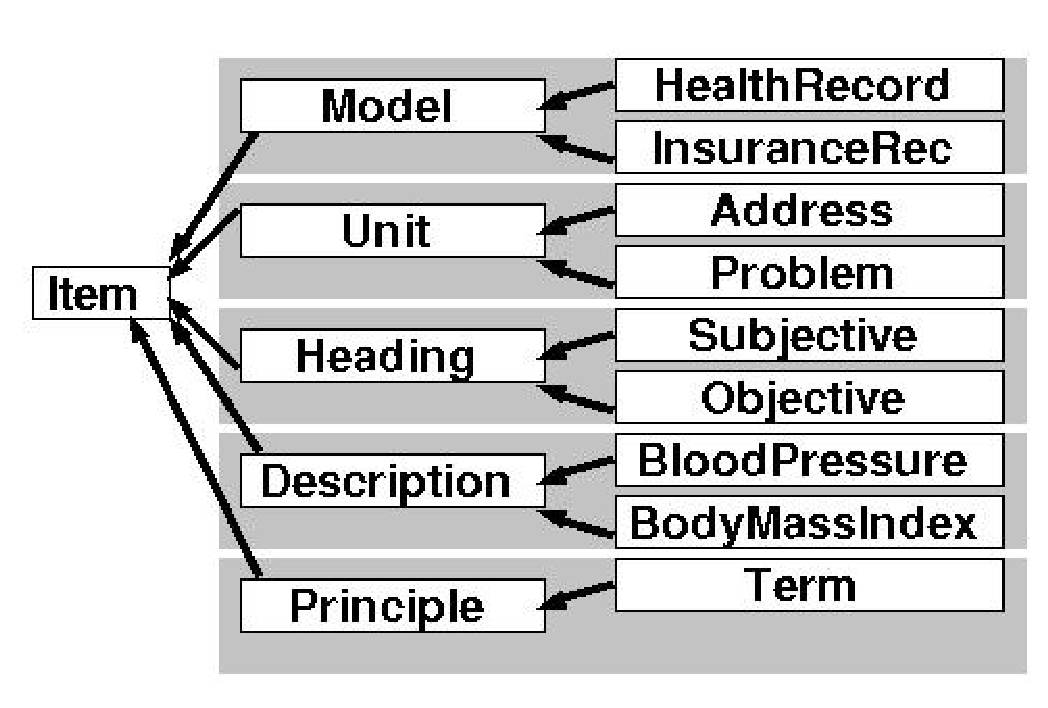
\includegraphics[scale=0.4]{vector/electronic_health_record_ontology.eps}
        \caption{Electronic Health Record Ontology}
        \label{electronic_health_record_ontology_figure}
    \end{center}
\end{figure}

Figure \ref{electronic_health_record_ontology_figure} shows one possible ontology
of an electronic health record, as described in the previous section.


    \section{CYBOP}
Section two introduced essential design patterns that represent
the main structure of the CYBOP framework. Section three explained the
Component Lifecycle and section four the well-known idea of ontology.
Now these design principles and conceptual architectures will be combined
to comprise their advantages and to increase the demanded quality characteristics:
high flexibility and maintainability.\\
\emph{Structure by Hierarchy} -- this is the basic idea behind CYBOP.
Extending the concept of Hierarchical Model-View-Controller to whole
software architectures, CYBOP was designed to be the domain-independent
backbone for information systems of any kind. Originally designed for
medical purposes, it should also be usable for insurance, financial or any
other standard applications in future.

\subsection{Class Item}
As shown, tree-like structures can be realized by the Composite pattern.
In CYBOP, this pattern can be found in class {\tt Item} which is super type
of all other classes. References, respectively relations to child elements
are held within a hashmap. No attributes were used except of this hashmap.
Every element of the map can be accessed by a special key value. So, no
particular {\tt get}- or {\tt set}-methods were needed for attributes.
\includepicture{6}{eps/item.eps}{Class Item}{Class Item}{Class Item}{Class Item}

\subsection{Basic Structure}
Comprising the design patterns \emph{Composite}, \emph{Layers}, and
\emph{Chain of Responsibility}, the framework CYBOP is comparable to a big
tree containing objects organized in different levels. Figure \ref{Basic Structure}
shows the object tree and the different levels of granularity.
\includepicture{8}{eps/framework-structure.eps}{Basic Structure}{Basic Structure}{Basic Structure}{Basic Structure}

    %
% $RCSfile: record.tex,v $
%
% Copyright (c) 2001-2004. Christian Heller. All rights reserved.
%
% Permission is granted to copy, distribute and/or modify this document
% under the terms of the GNU Free Documentation License, Version 1.1
% or any later version published by the Free Software Foundation;
% with no Invariant Sections, with no Front-Cover Texts and with no Back-Cover
% Texts. A copy of the license is included in the section entitled
% "GNU Free Documentation License".
%
% http://www.cybop.net
% - Cybernetics Oriented Programming -
%
% http://www.resmedicinae.org
% - Information in Medicine -
%
% @author Christian Heller <christian.heller@tuxtax.de>
% @author Jens Bohl <info@jens-bohl.de>
%

\section{Record -- An EHR Module}
\label{record_an_ehr_module_heading}

The practical background for the application of CYBOP is \emph{Res Medicinae}
\cite{resmedicinae}. A modern clinical information system is the aim of all efforts
in this project. In future, it shall serve medical documentation, archiving,
laboratory work etc. \emph{Res Medicinae} is separated into single modules depending
on different tasks.\\
One of these modules is \emph{Record} -- an application for documenting medical
information (figure \ref{record_figure}). In addition to new documentation models,
it also contains a tool for topological documentation.

\begin{figure}[ht]
    \begin{center}
       \includegraphics[scale=0.3]{eps/screenshot.eps}
       \caption{Screenshot of Record \cite{urban}}
       \label{record_figure}
    \end{center}
\end{figure}

Starting from an overall view of the human body, it is possible to reach every
organ or region of the body in detail (figure \ref{topology_figure}).

\begin{figure}[ht]
    \begin{center}
       \includegraphics[scale=0.5]{eps/topology.eps}
       \caption{Excerpt from Topological Structure of Human Skeleton}
       \label{topology_figure}
    \end{center}
\end{figure}


    %
% $RCSfile: summary.tex,v $
%
% Copyright (c) 2001-2004. Christian Heller. All rights reserved.
%
% Permission is granted to copy, distribute and/or modify this document
% under the terms of the GNU Free Documentation License, Version 1.1
% or any later version published by the Free Software Foundation;
% with no Invariant Sections, with no Front-Cover Texts and with no Back-Cover
% Texts. A copy of the license is included in the section entitled
% "GNU Free Documentation License".
%
% http://www.cybop.net
% - Cybernetics Oriented Programming -
%
% http://www.resmedicinae.org
% - Information in Medicine -
%
% @author Christian Heller <christian.heller@tuxtax.de>
% @author Jens Bohl <info@jens-bohl.de>
%

\section{Summary}
\label{summary_heading}

Software design patterns are essential elements of frameworks. They can be
combined to comprise their advantages and to realize hierarchical structures.
These structures can be created and destroyed in the lifecycle of components.
In that lifecycle, object relations become more transparent and are easier to
control and to maintain.\\
Ontologies can help to model particular domains and to layer software. Every level
of these ontologies has a particular supertype, whereby these types depend on each
other by inheritance. This concept supports the modelling and logical separation
of software into hierarchical architectures. The granularity of the ontology
(number of ontological levels) can be adapted to particular requests.\\
By applying the new concepts introduced in this document, the quality of software
can be greatly increased. The time for building systems can be reduced to a minimum.
The clear architecture avoids common confusion as the systems grow.


    %
% $RCSfile: acknowledgements.tex,v $
%
% Copyright (c) 2001-2004. Christian Heller. All rights reserved.
%
% No copying, altering, distribution or any other actions concerning this
% document, except after explicit permission by the author!
% At some later point in time, this document is planned to be put under
% the GNU FDL license. For now, _everything_ is _restricted_ by the author.
%
% http://www.cybop.net
% - Cybernetics Oriented Programming -
%
% http://www.resmedicinae.org
% - Information in Medicine -
%
% @author Christian Heller <christian.heller@tuxtax.de>
%

\section{Acknowledgements}
\label{acknowledgements_heading}

Our special thanks go to all Enthusiasts of the Open Source Community who have
provided us with a great amount of knowledge through a comprising code base to
build on. We'd also like to acknowledge the contributors of \emph{Res Medicinae},
especially all medical doctors who supported us with their analysis work
\cite{resmedicinae2001} and specialised knowledge in our project mailing lists.
Further on, great thanks goes to the Urban and Fischer publishing company, for
providing anatomical images from their \emph{Sobotta -- Atlas der Anatomie}.


    \label{references_heading}
    \bibliographystyle{geralpha}
    \bibliography{references}
\end{document}

